\chapter{Experiment}\label{sec:exp}

\section{Hardware Settings}

Our experimental environment consists of one master node and ten working nodes.
The master node is a physical machine with two quad-core CPU.
The CPU model is Intel(R) Xeon(R) CPU X5570 @ 2.93GHz.
On the other hand, each working node is a single-core physical machine.
The memory sizes are 1.5GB and 768MB, respectively.
Our management system works on the master node.
The master node also serves as a client which generate the workloads.
There are two workers on each working node.

\section{Worker Failure Tolerance}

\begin{figure}
  \resizebox{\columnwidth}{!}{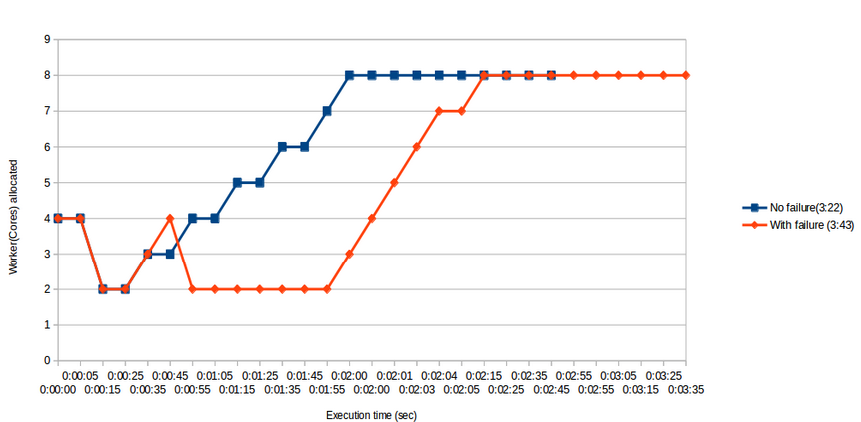
\includegraphics{figures/adaptive}}
  \caption{Worker Instance Allocation}
  \label{figure:worker-failure}
\end{figure}

We reproduced a small scale workload trace provided by Chunghwa Telecom
Laboratories~\cite{cite:cht-lab}.
Total of 8 worker instance is used and deadline-based scheduling policy
is applied in this simulation. 
1 job was sent and the deadline is set to 4 minutes.
The characteristic of this workload is that it starts with several
light-weight tasks and then comes with heavier tasks.

Figure~\ref{figure:worker-failure} shows the worker allocated for that
job.
The blue line is the normal execution, and the red line shows the
execution progress with workers manually shutted down to simulate worker
failure.
Six workers are manually shutted down at 0:00:55 and resumed after
0:01:55, which means at the period, only 2 workers are available.

We will discuss the normal execution (blue-line) first.
At the beginning, since we don't have any run time information, the
scheduler just use the default value (4 workers).
After few seconds, some tasks are done and the run time statistics from
\emph{status checker} shows that it seems that each task execution
progress is going faster than expected, so the system decided to
decrease the number of scheduled workers.
However, the system later found that the task execution progress had
been slowing down and current allocation might not be able to meet the
deadline, so it schedules more workers to the job.

The simulation with worker failure is similar to the normal one except
for we manually shutted down and resumed workers.
After worker resumed, the system tried harder to catch up the deadline.
We can see that the slope of the worker number change of red line is
greater than the blue line, implying the systems ability to adapt to
failure events.

\section{Trace-based Simulation}

We conducted a trace-based simulation to demonstrate the efficiency of
our system.
Since we cannot obtain traces with deadline, we decided to use traces in
{\em standard workload format}~\cite{cite:swf}.
The trace we used is the {\em CERIT-SC workload log}, which is provided
by the CERIT-SC and the Czech National Grid Infrastructure
MetaCentrum~\cite{cite:metacentrum}.
The data set containing 17,900 jobs are generated from TORQUE traces
during the first 3 months of the year 2013.
We took samples from these eighteen-thousand jobs, and scaled the
waiting and execution time of the sampled jobs.

\subsection{Simulation Settings}

The trace is however very sparse and skewed.
If we directly sample 1 percent of jobs the waiting time between jobs
can be extremely long --- maybe up to hours.
Because of this, we instead sample consecutive jobs only and scaled the
waiting time between jobs.
Limiting the number of jobs to sample out, we randomly pick a starting
job and take jobs consecutively after it. 
The sample rate is 0.01 and the scale factor of waiting time between
jobs is 0.1.

On the other hand, the running time distribution of the trace is very
long-tailed and more like a exponential distribution: Enormous number of
jobs has extremely short running time (several seconds), while some jobs
takes extremely long time (several days).
Therefore, we scaled down the running time of jobs by factor of 0.001.

There are still some assumptions to be made to fit our usage model.
First, we cannot obtain information about subtasks of a jobs.
So we take the processors of allocated for a job as its number of tasks
and take the total running time as the execution time of each task.

Besides, the information about batches, priority and deadlines is absent
in the trace but however our targeted characteristics.
Since jobs in standard workload format traces are independent,
we group jobs that will be submitted within 1 second together to
simulate batches.
For priority, we group jobs with same user IDs as same priority and we
give the priority group with less jobs higher priority.
As for the deadlines, we use the double of its running time as deadline
for those jobs with less than 4 tasks, and for those jobs with more
tasks, we use $2 * runtime * \#task / 4$ as deadline.

During simulation, the client starts new jobs according to the arrival
time and execution time from the trace.
Since the actual workloads is not available, a worker will be set to
``sleep mode'' after receiving a task from the client.
The sleeping duration is equal to the task execution length.
After resumed from the sleeping mode, the worker sends a message to the
management system indicating it has finished a task.

\subsection{Experiment Results}
\begin{figure}[htbp]
  \centering
  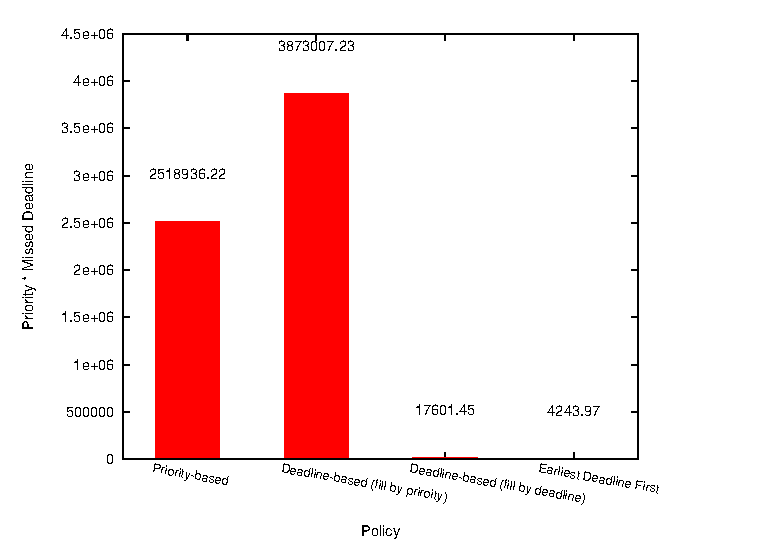
\includegraphics[width=\textwidth,height=0.7\textheight,keepaspectratio]{figures/homo.eps}
  \caption{Homogeneous Environment Setting}
  \label{fig:homo-result}
\end{figure}

\begin{figure}[htbp]
  \centering
  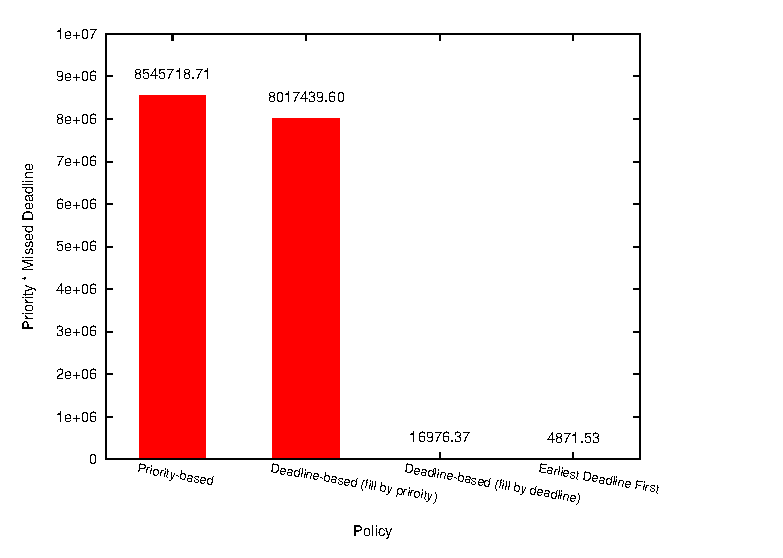
\includegraphics[width=\textwidth,height=0.7\textheight,keepaspectratio]{figures/hetero.eps}
  \caption{Heterogeneous Environment Setting}
  \label{fig:hetero-result}
\end{figure}
